\chapter{Introduction}
\label{cha:introduction}

This chapter provides the necessary background material and details the organization of my proposed work.

\section{What is context ?}
In computer vision, context \cite{contextvision} refers to any relevant information encompassing the attributes of the object and event considered, along with other entities (objects and events) in the given scene, both visual and non-visual. Contextual information enables a wide variety of tasks, including object recognition and salient event detection in videos, by providing additional cues needed for accurate inference. For example, the visual scene in a given image provides the necessary contextual information to detect commonly co-occurring objects along with any atypical placements. In terms of object placements, utensils are more likely to be found in the kitchen as compared to bedrooms or stadium. The broad organization of different context sources along with associated levels in Fig \ref{Context_type}.
\begin{figure}[t]
  \centering
  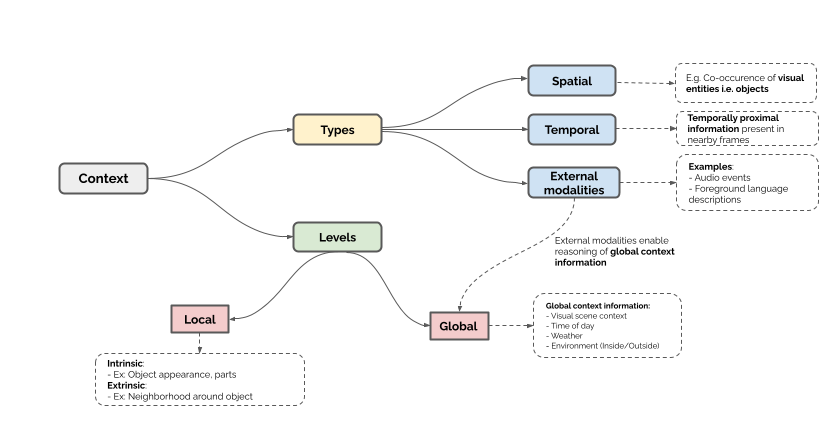
\includegraphics[width=\linewidth]{figures/Context_type.png}
  \caption{Variations in types and levels of context}
  \label{Context_type}
\end{figure}
\section{Multi-modal content}
\section{Context-driven multi-modal understanding}
\section{Organization of proposal}

